\documentclass{beamer}


\usepackage{graphicx, xcolor}
\usepackage{amsmath}
\usepackage{amsfonts}
\usepackage{lmodern}
\usepackage{listings}

\usetheme{Rochester}
\usepackage{minted}
\definecolor{bg}{rgb}{0.95,0.95,0.95}
\usepackage{graphics}
\usepackage{trfsigns}

\definecolor{mGreen}{rgb}{0,0.6,0}
\definecolor{mGray}{rgb}{0.5,0.5,0.5}
\definecolor{mPurple}{rgb}{0.58,0,0.82}
\definecolor{backgroundColour}{rgb}{0.92,0.92,0.92}


\lstdefinestyle{CStyle}{
	backgroundcolor=\color{backgroundColour},   
	commentstyle=\color{mGreen},
	keywordstyle=\color{magenta},
	numberstyle=\tiny\color{mGray},
	stringstyle=\color{mPurple},
	basicstyle=\fontsize{8}{7}\selectfont\ttfamily,
	breakatwhitespace=false,         
	breaklines=true,                 
	captionpos=b,                    
	keepspaces=true,                 
	numbers=left,                    
	numbersep=5pt,                  
	showspaces=false,                
	showstringspaces=false,
	showtabs=false,                  
	tabsize=2,
	language=C
}

\usepackage[absolute,overlay]{textpos}
\newenvironment{reference}[2]{%
  \begin{textblock*}{\textwidth}(#1,#2)
    \footnotesize\it\bgroup\color{blue!50!black}}{\egroup\end{textblock*}}

\setbeamertemplate{navigation symbols}{}



\title{CPFSK Softwareradio}
\author{Lukas Becker, Tobias Frahm}
\institute[HAW]{Dept. Informations- und Elektrotechnik\\HAW Hamburg}
\date{\today}


%\frame{
%  \frametitle{FIR-Polyphasen Bandpass}
%  \begin{columns}
%    \begin{column}{0.5\textwidth}
%
%    \end{column}
%    \begin{column}{0.5\textwidth}
%
%    \end{column}
%  \end{columns}
%}

\begin{document}

\frame[plain]{\titlepage}

\section[Outline]{}

\frame{\tableofcontents}

\section{Softwareradio}

\frame{
  \frametitle{Softwareradio}
  \begin{itemize}
  \item<1-> Was ist der Unterschied zu einem normalen Empfänger?
  \end{itemize}
}

\section{Signalfluss Empfänger}
\frame{
  \frametitle{Signalfluss Empfänger}
  \begin{columns}
    \begin{column}{0.3\textwidth}
       \begin{itemize}
         \item 1. FIR-Polyphasen Bandpass
         \item 2. komplexes Kammfilter
         \item 3. FM-Verzögerungsdemodulator
         \item 4. Decodierer
       \end{itemize}
    \end{column}
    \begin{column}{0.7\textwidth}
        \begin{center}
         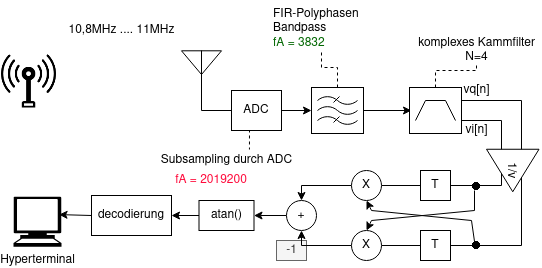
\includegraphics[width=0.6\textwidth]{images/signalfluss.png}
         \end{center}
    \end{column}
  \end{columns}
}
\section{FIR-Polyphasen Bandpass}
\frame{
  \frametitle{FIR-Polyphasen Bandpass}
  \begin{columns}
    \begin{column}{0.5\textwidth}
      \begin{itemize}
        \item in MATLAB Bandpass als FIR-Filter ausgelegt
        \item Dezimationsfaktor bestimmt
        \item Mit Pyhton einen C-Headerfile mit den Polyphasen erzeugt.
      \end{itemize}
    \end{column}
    \begin{column}{0.5\textwidth}
        \begin{itemize}
          \item performanter ANSI-C Code durch Pointerarithmetik
          \item und vermeidung von Schleifen
        \end{itemize}
    \end{column}
  \end{columns}
}

\subsection{FIR Bandpass in MATLAB}
\frame{
  \frametitle{FIR Bandpass in MATLAB}
  \begin{columns}
    \begin{column}{0.5\textwidth}
      Iteratives Vorgehen bis die Koeffizientenanzahl 
      annehmbar war.
      \begin{itemize}
        \item Festlegung der Grenzfrequenzen $f_u = 3800Hz$ und $f_o = 4500Hz$
        \item Abschätzen der Start-/Stopfrequenzen $f_{start/stop} = f_{u/o} \pm 1500Hz$.
      \end{itemize}
    \end{column}
    \begin{column}{0.5\textwidth}
      Bei dem hier gezeigten Amplitudengang werden 2056 Koeffizienten benötigt.
      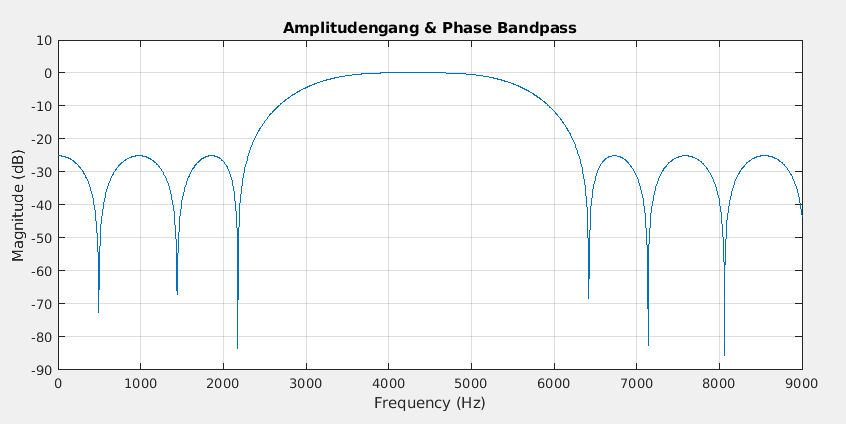
\includegraphics[width=\textwidth]{images/FIR_BP.png}
    \end{column}
  \end{columns}
}

\subsection{FIR-Polyphasen Bandpass in ANSI-C}
\frame{
  \frametitle{FIR-Polyphasen Bandpass in ANSI-C}
  \begin{columns}
    \begin{column}{0.5\textwidth}
      Zunächst werden die Koeffizienten des FIR-Bandpass exportiert.
      Anschließend mithilfe eines Pythonscripts in $527$ Polyphasen
      aufgeteilt, ggf. mit nullen aufgefüllt, und als \textit{const char}-Arrays
      in ein C-File exportiert.
    \end{column}
    \begin{column}{0.5\textwidth}
      \begin{itemize}
        \item \textit{const char} für effiziente Speichernutzung
        \item effizienter Zugriff nur durch Pointerreferenz
      \end{itemize}
    \end{column}
  \end{columns}
}

\frame{
  \frametitle{FIR-Polyphasen Bandpass in ANSI-C}
  \begin{columns}
    \begin{column}{0.5\textwidth}
      \begin{itemize}
        \item Die Dezimationsstufen werden in einem Array gespeichert
        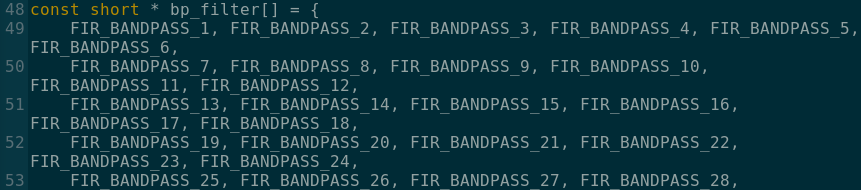
\includegraphics[width=0.9\textwidth]{images/bp_filter.png}
        \item Die einzelnen Stufen, werden nach und nach dem FIR übergeben.
        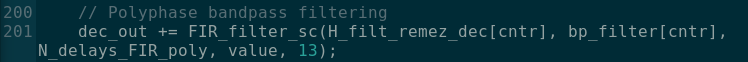
\includegraphics[width=0.9\textwidth]{images/FIR_call.png}
      \end{itemize}
    \end{column}
    \begin{column}{0.5\textwidth}
      Bild Ausgang Bandpass
    \end{column}
  \end{columns}
}

\section{Hilbert Transformator}

\frame{
  \frametitle{Hilbert Transformator}
  \begin{columns}
    \begin{column}{0.5\textwidth}
      
    \end{column}
    \begin{column}{0.5\textwidth}
      Bild Ausgang Bandpass
    \end{column}
  \end{columns}
}

\section{Komplexes Kammfilter}
\frame{
  \frametitle{Komplexes Kammfilter}
  \begin{columns}
    \begin{column}{0.5\textwidth}
      Auslegung
      \begin{itemize}
        \item festlegen des Abstandes von HP zu Nullstelle
        \item Anzahl der Verzögerer bestimmen.
        \item Nullstelle auf $w_{mark/space}$ verschieben
      \end{itemize}
    \end{column}
    \begin{column}{0.5\textwidth}
      \begin{itemize}
        \item $H(jwu) = 1 + e^{jwu}$ mit $w =  \frac{\varDelta f}{fA}$
        \item $ u = \lfloor \frac{\pi}{2 \pi \frac{\varDelta f}{fA}} \rfloor = 4$
        \item $ h(k) \cdot e^{-j\omega_{space}\cdot k}$
        \item $h(k) = \{ 1, 0, 0, 0, 0.175 + i0.985\}$
       \end{itemize}
      \end{column}
  \end{columns}
}

\frame{
  \frametitle{Komplexes Kammfilter}
  \begin{columns}
    \begin{column}{0.3\textwidth}
      
      \begin{itemize}
        \item jeweils eine Frequenz wird gedämpft
        \item Nullstellen sind verschoben
        \item es ensteht ein komplexes Signal
      \end{itemize}
    \end{column}
    \begin{column}{0.7\textwidth}
      Amplitudengang
      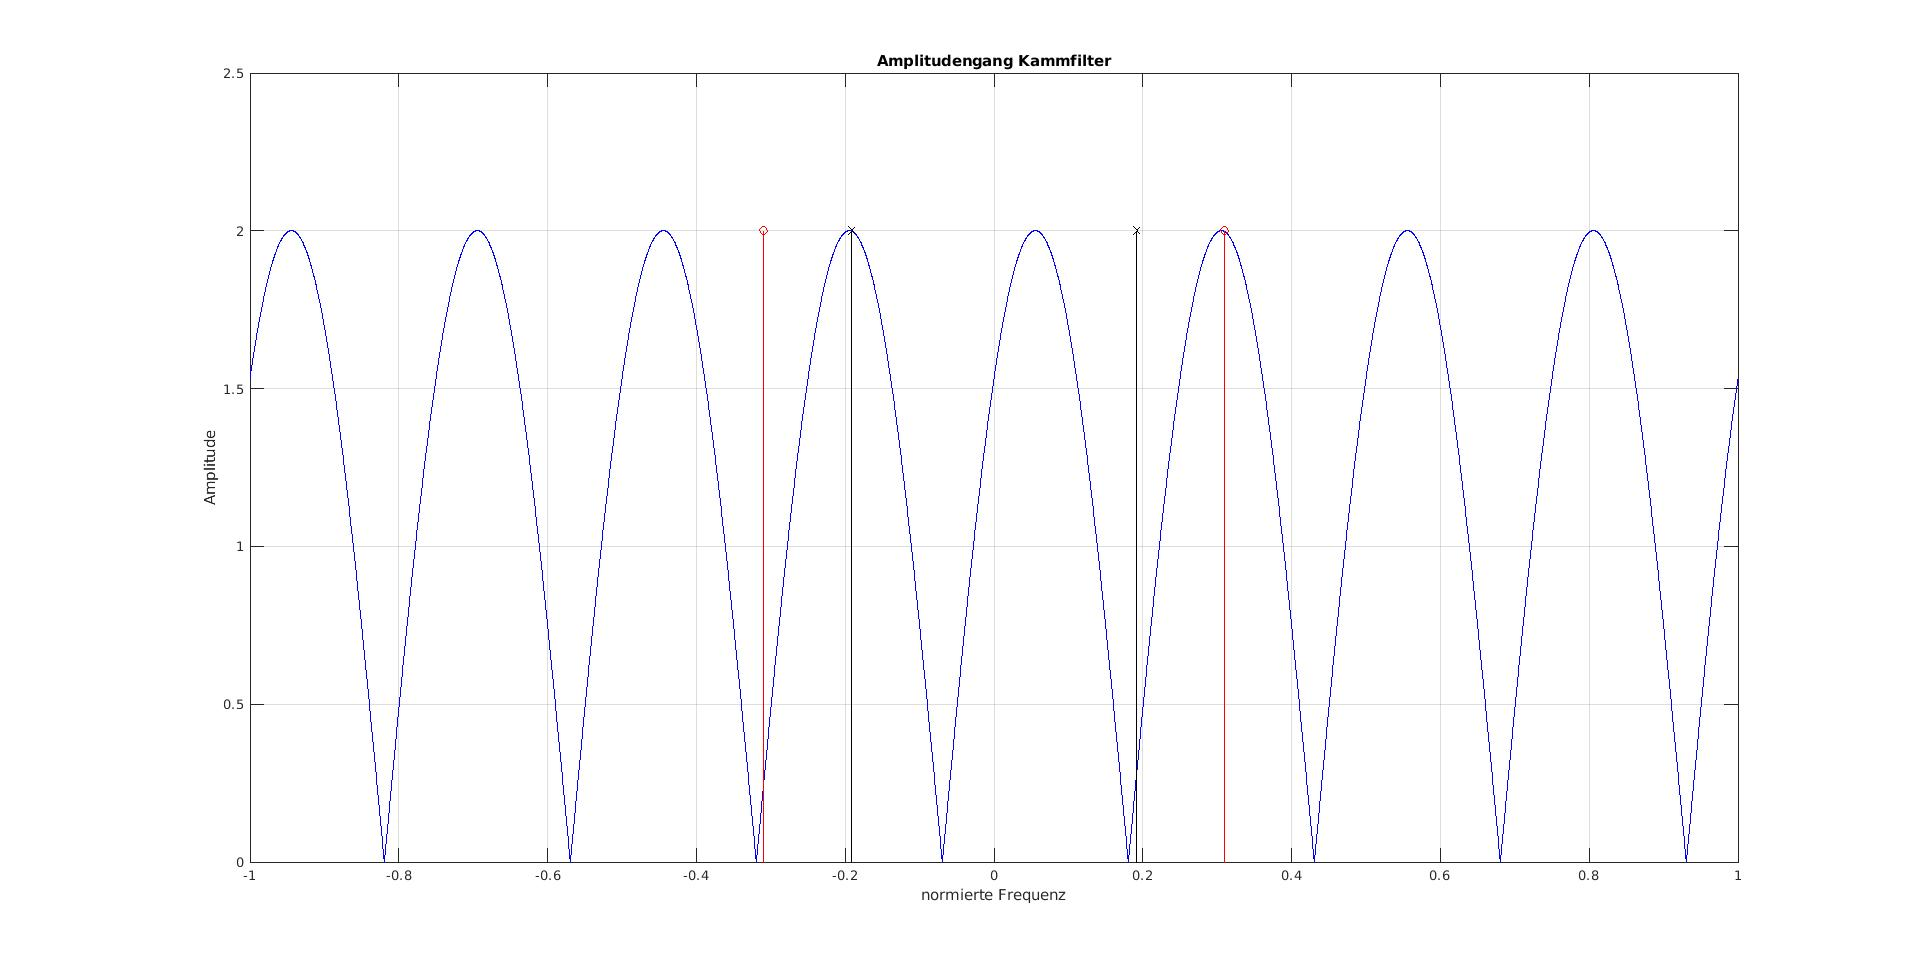
\includegraphics[width=\textwidth]{images/comb.png}
      \end{column}
  \end{columns}
}

\section{FM-Verzögerungsdemodulator}
\section{Dekodierer}
\frame{
  \frametitle{Decodierer}
  \begin{columns}
    \begin{column}{0.5\textwidth}
      \begin{itemize}
        \item Demodulierte Rechtecksignal als Bitstream
        \item Lookuptable
        \item Wechsel zwischen Nummern und Buchstaben durch austauschen der Lookuptable
      \end{itemize}
    \end{column}
    \begin{column}{0.5\textwidth}
        \begin{itemize}
          \item Weiteres mal Unterabtasten ca.$38Hz$
          \item Pointerarithmetik
          \item Aus Bitstream wird direkt ein Index erreichnet
          \item keine Schleifen
        \end{itemize}
      \end{column}
  \end{columns}
}
\frame{
  \frametitle{Decodierer - Matlab}
  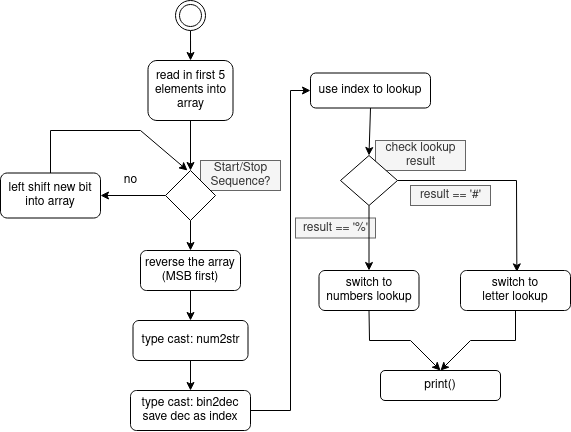
\includegraphics[width=0.9\textwidth]{images/matlab-lookup.png}
}


\frame{
	\frametitle{Theorie Dekodierer}
	
	\begin{figure}
		\centering
		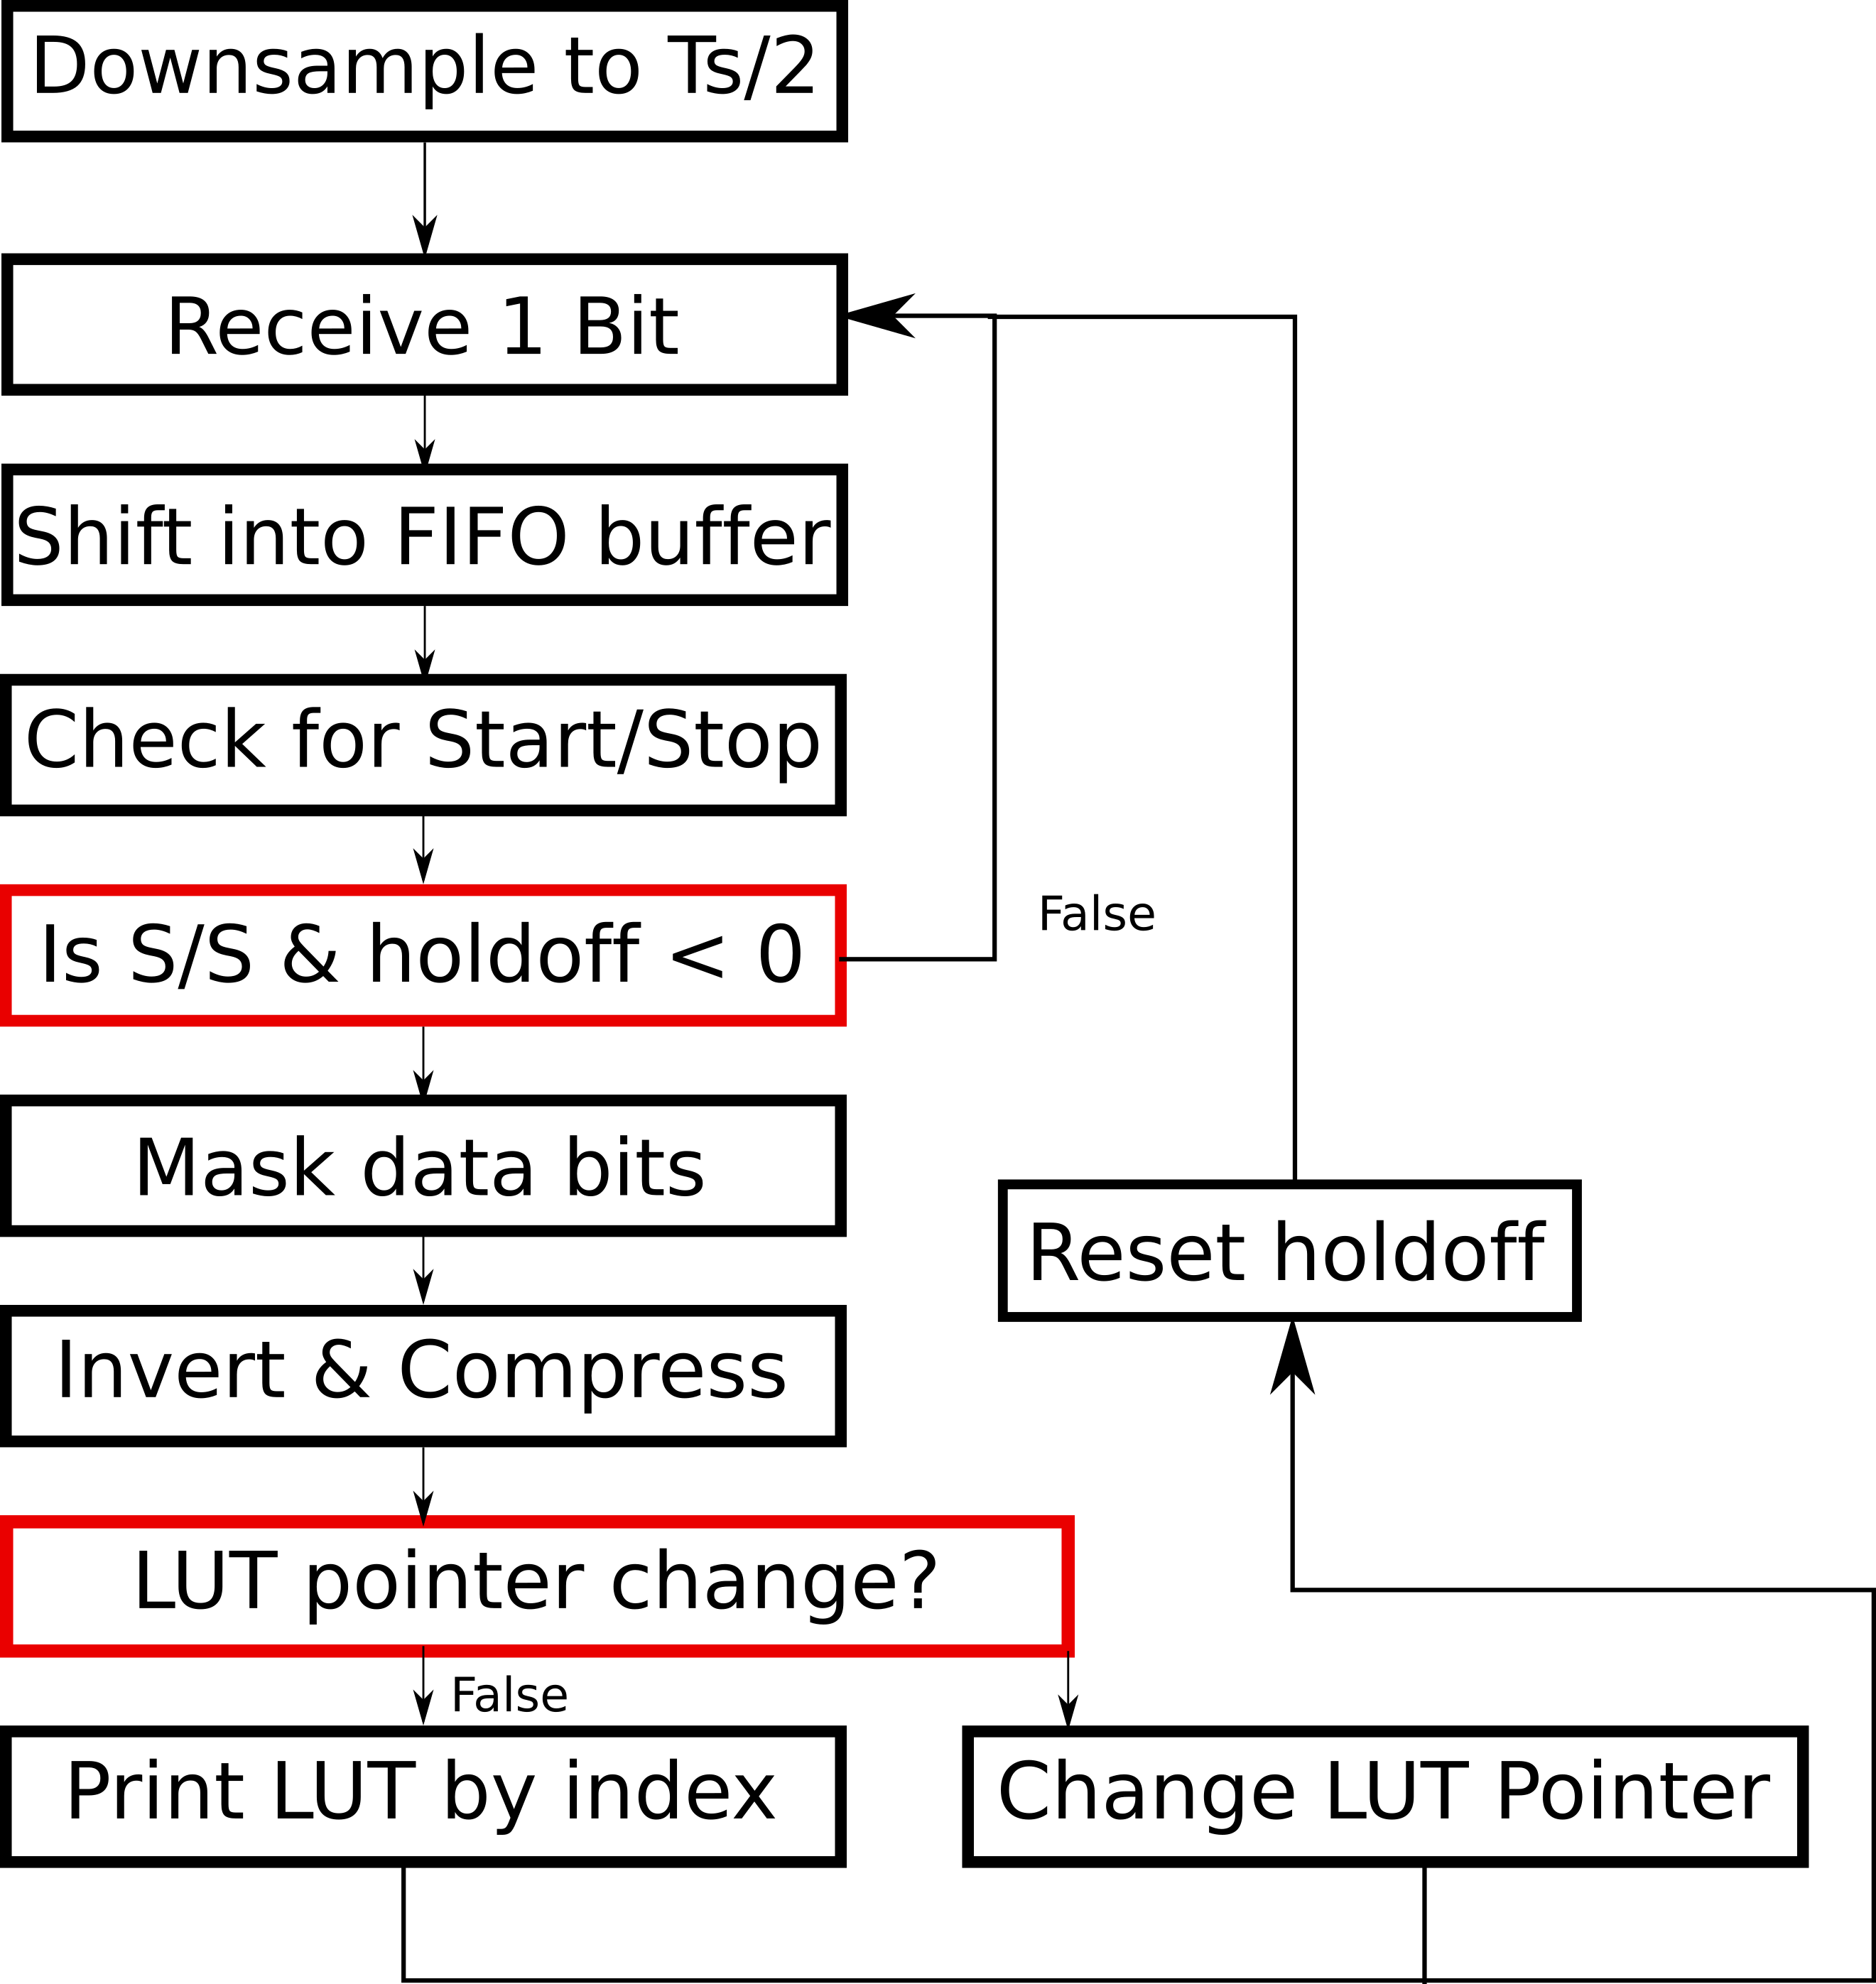
\includegraphics[width=0.7\linewidth]{images/rect833}
		\caption{}
		\label{fig:rect833}
	\end{figure}
	
}


\begin{frame}[fragile]
	\frametitle{Implementierung Dekodierer}
	
	\begin{lstlisting}[basicstyle=\tiny,style=CStyle]			
buffer = buffer << 1; // Shift FIFO left
buffer = buffer | bit; // Enter bit
startstop = buffer & 0x001F; // Mask size of start/stop

if (startstop_holdoff > 0) // Underflow protection
	startstop_holdoff -= 1;

if (startstop == STOP_SEQUENCE && startstop_holdoff == 0) {
	startstop_holdoff = 11;
	index_pre = (buffer >> 5) & 0x03FF; 
	real_index =  (((index_pre >> 0) & 0x0001) << 4) 
		   		   	| (((index_pre >> 2) & 0x0001) << 3) 
							| (((index_pre >> 4) & 0x0001) << 2) 
							| (((index_pre >> 6) & 0x0001) << 1) 
							| (((index_pre >> 8) & 0x0001) << 0);

	if (real_index == SWITCH_TO_CHAR) {
		current_lut = lookup_char;
	} else if (real_index == SWITCH_TO_NUM) {
		current_lut = lookup_num;
	} else {
		printf(" >> %c <<\n",current_lut[real_index-1]); 
	}
}

\end{lstlisting}
\end{frame}

\nocite{*} % Include everything in the .bib file.

\bibliographystyle{plainnat}
\bibliography{presentation}

% that's all, folks
\end{document}
